\documentclass[journal]{IEEEtran}

\usepackage{amsmath,amssymb,bm}
\usepackage{booktabs}
\usepackage{graphicx}
\usepackage{cite}
\usepackage{array}
\usepackage{multirow}
\usepackage{xcolor}
\usepackage{url}
\usepackage{microtype}

\graphicspath{{figures/}}

\newcommand{\R}{\mathbb{R}}
\newcommand{\E}{\mathbb{E}}
\newcommand{\ind}{\mathbb{I}}
\newcommand{\TODO}[1]{\textbf{[TBD: #1]}}
\DeclareMathOperator{\CVaR}{CVaR}

\begin{document}

\title{Availability-Aware Weak-Physics Residual Flow Matching for Joint Wind-Power Scenarios and Ramp-Risk Assessment}

\author{\TODO{First Author}, \TODO{Coauthors}, and \TODO{Corresponding Author}%
\thanks{Manuscript prepared for possible submission to IEEE Transactions on Sustainable Energy. Author names, affiliations, funding, and correspondence information must be inserted before submission.}%
}

\maketitle

\begin{abstract}
Reliable ultra-short-term wind-power forecasting requires more than a point trajectory: operators also need coherent future scenarios, calibrated uncertainty ranges, and traceable ramp-risk indicators. This paper presents PR-Warn++, an availability-aware framework that separates these predictive objects. A monotone empirical power curve fitted only on valid training observations provides a weak physical anchor. A mask-aware temporal multi-graph network then predicts the remaining deterministic residual from rigid-grid SCADA histories, observation masks, elapsed-time features, and geographic, statistical, directional, and adaptive dependencies. Conditional flow matching is applied only after this stage and directly models the joint turbine-by-horizon final forecast-error field, avoiding a primary VAE bottleneck and avoiding the need to regenerate the predictable power trend. The resulting joint scenarios support three deliberately separate assessments: multivariate scenario fidelity, per-horizon marginal interval calibration, and event/tail-risk reliability. Split conformal prediction is used only for the marginal coverage claim, while ramp, deviation, and conditional value-at-risk quantities are derived from farm-level scenarios as wind-side operational proxies. Evaluation is designed around a strict history-only SDWPF protocol, with retrospective ERA5 and auditable issue-time weather studied separately. \TODO{Insert only server-validated quantitative results.}
\end{abstract}

\begin{IEEEkeywords}
wind power forecasting, probabilistic forecasting, flow matching, conformal prediction, spatio-temporal graphs.
\end{IEEEkeywords}

\section{Introduction}

Ultra-short-term wind-power forecasts are used to anticipate renewable variability over the next several dispatch intervals. For a large turbine array, however, a single expected trajectory does not reveal whether errors are spatially synchronized, whether a farm-level ramp is plausible, or how severe the lower tail may be. These questions require a joint predictive distribution over turbines and lead times rather than a collection of unrelated point forecasts. They are also sensitive to SCADA outages and operating-state changes. The SDWPF benchmark makes these difficulties visible at scale through 10-min measurements from 134 turbines, turbine locations, and contextual variables \cite{zhou2024sdwpf}.

Spatio-temporal graph forecasting has become a mature approach for representing turbine and site dependence. Recent work includes time-aware graph convolution for probabilistic wind forecasting \cite{tang2024timeaware}, graph Transformers with auto-correlation \cite{liang2025wpformer}, graph-contrastive robustness \cite{liu2025graphcontrast}, and dynamic matching under concept drift \cite{li2025dynamic}. Wind-speed/direction-aware inter-farm correlation graphs \cite{wang2025clustergraph} and wake-directed turbine graphs \cite{hou2026wake} further show the value of directional structure at different spatial scales. These advances motivate a multi-view graph backbone, but they also imply that a dynamic graph alone is no longer a sufficient novelty claim.

Probabilistic wind forecasting now spans marginal intervals, adaptive distributions, and scenario generation. TSTE and Applied Energy studies have addressed optimized prediction intervals \cite{chen2024interval}, meta-adaptation \cite{meng2024meta}, missing-data-tolerant probabilistic forecasting \cite{meng2026missing}, non-crossing spatio-temporal quantiles \cite{chen2025noncrossing}, and conformalized regional distributions \cite{jonkers2024conformal}. Diffusion models have recently generated wind-power or wind-speed trajectories \cite{liu2026diffusion,gao2026diffusion,ma2026stgld}. Therefore, neither interval calibration nor generative modeling is by itself the unresolved problem. The more specific question is \emph{which uncertainty object should be generated after a forecast-origin-valid deterministic model has already absorbed the predictable structure}.

Physics and weather inputs sharpen this question but also create an information-boundary risk. Power-curve knowledge and physics-informed learning can improve robustness \cite{gao2025tgdpF,liu2024physicsrl}. Separate studies address overlapping NWP products, weather transitions, and wide-area meteorological representations \cite{zhao2025nwp,zhang2026transitional,cao2026joint}. Yet a retrospective weather field is not interchangeable with a forecast issued before the prediction origin. In SDWPF-full, future ERA5 is retrospective reanalysis intended to separate meteorological forecast error from the power-forecasting task \cite{zhou2024sdwpf}. Using it silently in the main protocol would turn an oracle experiment into an apparently operational forecast.

Three gaps follow. First, graph and physics-guided models are commonly optimized as final predictors, whereas generators often model raw future power. This leaves the joint \emph{final forecast-error field} after a structured deterministic center underexplored. Second, a model may produce realistic multivariate scenarios while retaining biased marginal intervals, and marginal conformal coverage does not calibrate nonlinear ramp-event probabilities. Joint scenario quality, marginal coverage, and event-probability reliability must therefore be evaluated separately. Third, deletion or interpolation of abnormal timestamps and unqualified use of future weather can hide deployment-invalid information. A useful probabilistic model must make availability and degradation paths auditable.

PR-Warn++ addresses these gaps with the decomposition
\begin{equation}
\bm Y_t=\bm P^{\rm pc}_t+\bm R_t,
\qquad
\bm Y_t=\hat{\bm Y}^{\rm det}_t+\bm E_t,
\label{eq:two_residuals_intro}
\end{equation}
where the two residuals have different roles. $\bm R_t$ is the deterministic structure not explained by the weak power-curve anchor, whereas $\bm E_t$ is the stochastic error left after the complete deterministic predictor. The framework uses a temporal multi-graph model for $\bm R_t$ and direct conditional flow matching (CFM) for $\bm E_t$. Generated joint error fields are added to the unchanged deterministic center to obtain coherent scenarios. Marginal conformal intervals and scenario-derived wind-side risk proxies are then produced through separate post-processing paths.

The contributions are summarized as three methodological contributions plus one supporting protocol contribution.
\begin{itemize}
\item \textbf{Availability-aware weak-physics residual center:} a training-only monotone empirical power curve is used as an auditable anchor, while rigid-grid masks and elapsed-time features enter a temporal multi-graph residual forecaster. The contribution is the decomposition under an explicit information boundary, not a claim that the empirical curve is a complete wake model.
\item \textbf{Direct joint generation of final forecast errors:} standard CFM models $p(\bm E_t\mid\mathcal I_t)$ after the deterministic center. This makes deterministic error reduction and stochastic dependence modeling separately testable. VAE-CFM and explicit minibatch optimal-transport pairing are retained only as controlled ablations.
\item \textbf{Separated reliability objects:} joint scenario fidelity, per-horizon marginal interval coverage, and ramp/deviation probability reliability are evaluated with different metrics and claims. Conformal calibration is not used as evidence that the entire joint scenario distribution or nonlinear event probabilities are calibrated.
\item \textbf{Auditable degradation and weather protocols:} the main history-only experiment, retrospective ERA5 oracle, and true issue-time weather protocol are isolated. Missingness and extreme-regime stresses preserve the rigid grid and never present future truth as an online input.
\end{itemize}

\section{Related Work}

\subsection{Availability-Aware Spatio-Temporal and Weak-Physics Forecasting}

Graph-based wind forecasting now covers static, adaptive, and time-varying dependence. Time-aware graph convolution \cite{tang2024timeaware}, adaptive graph perception \cite{yang2024gcn}, graph Transformers \cite{liang2025wpformer}, and contrastive graph learning \cite{liu2025graphcontrast} all demonstrate the importance of spatial structure. Dynamic matching addresses temporal drift \cite{li2025dynamic}, while missing-data-tolerant probabilistic forecasting treats incomplete observations as part of the modeling problem rather than a purely offline cleaning issue \cite{meng2026missing}. More generally, GRU-D showed that an observation mask and time since last observation can carry predictive information that is lost by plain imputation \cite{che2018grud}.

Physics-guided wind forecasting ranges from power-curve regularization to detailed wake models. Power-curve knowledge has been integrated into noise-resilient deep forecasting \cite{gao2025tgdpF}, and physics-informed probabilistic learning has been studied for extreme events \cite{liu2024physicsrl}. At the wind-farm-cluster scale, wind speed and direction have been used to construct correlation graphs \cite{wang2025clustergraph}; at the turbine scale, a physical cone can define a wake-oriented directed graph \cite{hou2026wake}. PR-Warn++ deliberately occupies a weaker but more auditable point on this spectrum: it uses a train-only empirical curve and a directional/advection prior, without presenting either as a calibrated aerodynamic wake solver. This choice matches the variables and identifiability available in the main benchmark.

\subsection{Probabilistic Forecasting and Joint Scenario Generation}

Marginal uncertainty methods include prediction-interval optimization \cite{chen2024interval}, meta-learning across conditions \cite{meng2024meta}, non-crossing quantile models \cite{chen2025noncrossing}, and conformalized predictive systems \cite{jonkers2024conformal}. They provide important baselines for sharpness and marginal reliability, but independently estimated quantiles do not necessarily preserve cross-turbine and cross-horizon dependence.

Generative models instead treat a future trajectory or field as one predictive object. Transformer diffusion has been used for spatio-temporal wind-speed distributions \cite{liu2026diffusion}; conditional diffusion and graph latent diffusion have been used for wind-power and regional wind-speed scenarios \cite{gao2026diffusion,ma2026stgld}. Flow matching learns a continuous vector field between a simple base law and a data law through regression \cite{lipman2023fm}, and recent time-series work demonstrates its forecasting potential \cite{kollovieh2025tsflow}. The distinct hypothesis in PR-Warn++ concerns the target, not the mere use of a generator: under a common conditioner and capacity, generation of raw power $\bm Y$, power-curve residual $\bm R$, and final error $\bm E$ are compared directly.

\subsection{Calibration, Distribution Shift, and Wind-Side Risk}

Conformal prediction can convert a base interval into a finite-sample marginal coverage statement under its stated calibration assumptions. Conformalized quantile regression supplies the asymmetric interval-score construction used here to wrap scenario-derived quantiles \cite{romano2019cqr}, while adaptive conformal inference updates the miscoverage level over a chronological stream \cite{gibbs2021aci}. These guarantees must not be overstated: per-horizon coverage over calibration-compatible origins is not simultaneous coverage over every turbine and horizon, nor does it calibrate an arbitrary nonlinear event functional of a joint trajectory.

Operationally oriented studies forecast ramp rates directly \cite{ko2026ramp} or define application-centered risk regions \cite{yang2025risk}. PR-Warn++ follows a scenario-to-risk route instead. Farm-level ramp and deviation probabilities and tail shortfalls are Monte Carlo functionals of the same joint scenarios and are evaluated with Brier score, reliability diagnostics, AUPRC, and realized losses. Without a network, dispatch, and reserve model, these quantities remain wind-side proxies rather than line-flow, voltage, frequency, or reserve-security probabilities.

The literature therefore motivates a connected but claim-separated design: availability-aware deterministic structure, joint generation of what remains, marginal interval calibration, and event/tail evaluation. Section III defines that design and its forecast-origin information set.

\section{Problem Formulation and Proposed Framework}

Fig.~\ref{fig:framework} summarizes the complete forecast-origin, training-target, calibration, and evaluation paths of the proposed framework.

\subsection{Forecast-Origin Information Set and Protocols}

Consider $N$ turbines observed on a rigid 10-min grid. At forecast origin $t$, the previous $L$ intervals are used to predict the next $H$ intervals. Let
\begin{align}
\bm X_t&\in\R^{N\times L\times D}, &
\bm M_t&\in\{0,1\}^{N\times L\times D},\nonumber\\
\bm\Delta_t&\in\R_+^{N\times L\times D}, &
\bm Y_t&\in\R^{N\times H},
\label{eq:tensors}
\end{align}
where $\bm M_t$ marks valid observations and $\bm\Delta_t$ records elapsed time since the last valid value. A reason code is retained beside the tensors to distinguish missing, invalid, curtailed, and other auditable states, but it is not silently converted into future information. The task is to estimate a deterministic center and the joint predictive law
\begin{equation}
p(\bm Y_t\mid\mathcal I_t),
\qquad
\mathcal I_t=\sigma\{Z:a(Z)\leq t\},
\label{eq:information_set}
\end{equation}
where $a(Z)$ denotes the observation or issue time of a candidate variable $Z$.

The primary \emph{history-only} protocol uses historical SCADA, static turbine metadata, and historical contextual variables available by $t$. Future ERA5 reanalysis is excluded. An \emph{oracle-weather} protocol may attach ERA5 at $t+1{:}t+H$, but is labeled retrospective and non-deployable. A third \emph{issue-time weather} protocol permits forecast fields only after an as-of join selects the latest issue timestamp not later than $t$. All scalers, power curves, correlation graphs, error normalizers, and calibration objects are fitted on their designated Train or Calib periods only.

\subsection{Rigid-Grid Availability Representation}

Invalid timestamps are preserved on the rigid grid. After Train-only standardization, numerical carriers $\tilde{\bm X}_t$ use last-observation carry-forward, with a Train median before the first valid value. A carrier is never presented alone. The actual temporal encoder receives
\begin{equation}
\bm U_t=\operatorname{concat}\!\left(
\tilde{\bm X}_t,\bm M_t,\log(1+\bm\Delta_t)
\right),
\label{eq:availability_input}
\end{equation}
so a carried value remains distinguishable from a fresh observation. Official dataset validity rules take precedence over optional outlier detectors. The reason-code sidecar supports auditing, subgroup evaluation, and controlled missingness stresses.

\subsection{Weak-Physics Deterministic Center}

Let $t_i^\star\leq t$ be the most recent valid wind-speed observation for turbine $i$. If pressure and temperature are available by the origin, dry-air density and reference-density wind speed are
\begin{equation}
\rho_{i,t_i^\star}=\frac{p_{i,t_i^\star}}{R_dT_{i,t_i^\star}},
\qquad
v^{\rm eq}_{i,t_i^\star}=v_{i,t_i^\star}
\left(\frac{\rho_{i,t_i^\star}}{\rho_0}\right)^{1/3};
\label{eq:density}
\end{equation}
otherwise the observed wind speed is used. The correction follows standard power-performance practice \cite{lee2020pcwg} and never requires future reanalysis in the main protocol.

A monotone empirical curve $f_{\rm pc}$ is fitted on valid Train normal-operation samples by wind-speed bin medians, weighted isotonic smoothing, interpolation, and clipping. The history-only anchor is persistent over the short horizon,
\begin{equation}
P^{\rm pc}_{i,t+h}=f_{\rm pc}(v^{\rm eq}_{i,t_i^\star}),
\qquad h=1,\ldots,H.
\label{eq:pc_anchor}
\end{equation}
It is an auditable reference, not a wind-speed forecast or a universal turbine model.

Four graph views describe complementary dependence. A Gaussian geographic graph is sparsified to the nearest neighbors,
\begin{equation}
A^{\rm geo}_{ij}\propto\exp(-d_{ij}^2/\sigma_d^2).
\end{equation}
A Train-only statistical graph uses the absolute pairwise correlation of first-differenced valid power and top-$K$ sparsification. With source-to-destination bearing $\beta_{ij}$ and forecast-origin wind direction $\theta_{i,t}$, the directional graph is
\begin{equation}
A^{\rm dir}_{ij}(t)\propto
e^{-d_{ij}/\lambda_d}
e^{-\delta(\beta_{ij},\theta_{i,t}+180^\circ)^2/(2\sigma_\theta^2)}
\ind_{\rm sector},
\label{eq:direction_graph}
\end{equation}
and is interpreted only as a directional/advection prior. A learned adaptive graph follows node-embedding constructions \cite{wu2019graphwavenet,bai2020agcrn},
\begin{equation}
\bm A^{\rm adp}=\operatorname{softmax}
\left(\operatorname{ReLU}(\bm E_1\bm E_2^\top)\right).
\end{equation}
The forecast-origin context produces gated mixture weights,
\begin{align}
\bm A_t&=\sum_{k\in\{\rm geo,corr,dir,adp\}}
\alpha_k(t)\bm A_t^{(k)},\nonumber\\
\bm\alpha_t&=\operatorname{softmax}(g_\theta(\bar{\bm H}_t)).
\label{eq:graph_mix}
\end{align}

Consistent with the implemented v3.2 backbone, temporal convolutions first encode $\bm U_t$. The last historical representation is then updated by residual graph blocks $\mathcal G_\ell$ using $\bm A_t$ and decoded to the deterministic residual,
\begin{align}
\bm H_t^{(0)}&=\operatorname{Last}\!\left(\operatorname{TCN}(\bm U_t)\right),\nonumber\\
\bm H_t^{(\ell+1)}&=\operatorname{LN}\!\left[\bm H_t^{(\ell)}+
\mathcal G_\ell(\bm H_t^{(\ell)};\bm A_t)\right],\nonumber\\
\hat{\bm R}_t&=\operatorname{Dec}_R(\bm H_t^{(G)}),\nonumber\\
\hat{\bm Y}^{\rm det}_t&=\operatorname{clip}\!\left(
\bm P^{\rm pc}_t+\hat{\bm R}_t,0,\bm P^{\rm rated}\right).
\label{eq:det_center}
\end{align}
The training target here is $\bm R_t=\bm Y_t-\bm P^{\rm pc}_t$. A masked Huber objective is used only on valid future targets. In the issue-time weather ablation, forecast weather and its availability mask are encoded separately and fused into the deterministic representation; no such tensor exists in the history-only main model.

\subsection{Direct CFM of the Final Forecast-Error Field}

After selecting the deterministic checkpoint, the generator target is
\begin{equation}
\bm E_0=\bm Y_t-\hat{\bm Y}^{\rm det}_t\in\R^{N\times H}.
\label{eq:final_error}
\end{equation}
This is not the power-curve residual in the previous subsection. A Train-only per-horizon standardizer produces $\bar{\bm E}_0$. For the primary independent-pair CFM, draw $\bm Z\sim\mathcal N(\bm0,\bm I)$ and $\tau\sim\mathcal U(0,1)$, and define
\begin{equation}
\bm E_\tau=(1-\tau)\bar{\bm E}_0+\tau\bm Z,
\qquad
\bm u_\tau=\bm Z-\bar{\bm E}_0.
\label{eq:cfm_path}
\end{equation}
A graph-conditioned velocity $v_\phi(\bm E_\tau,\tau,\bm H_t,\bm A_t)$ minimizes the masked regression loss
\begin{equation}
\mathcal L_{\rm CFM}=\frac{
\sum \bm M^Y_t\odot
\left\|v_\phi(\bm E_\tau,\tau,\bm H_t,\bm A_t)-\bm u_\tau\right\|_2^2}
{\sum \bm M^Y_t}.
\label{eq:cfm_loss}
\end{equation}
Missingness and optional issue-time weather affect the generator only through the forecast-origin deterministic representation and fused graph. The main method is standard CFM. A Hungarian minibatch assignment is enabled only in the explicit optimal-transport ablation; VAE-CFM is likewise a separate ablation rather than the primary path.

At inference, $M$ Gaussian fields are integrated from $\tau=1$ to $0$. The default implementation uses $K_{\rm step}$ reverse-Euler steps,
\begin{equation}
\bm E_{\tau-\Delta\tau}=\bm E_\tau-
\Delta\tau\,v_\phi(\bm E_\tau,\tau,\bm H_t,\bm A_t).
\label{eq:reverse_ode}
\end{equation}
After inverse standardization, the unchanged center reconstructs the scenarios,
\begin{equation}
\bm Y_t^{(m)}=\operatorname{clip}\!\left(
\hat{\bm Y}^{\rm det}_t+\bm E_0^{(m)},0,\bm P^{\rm rated}
\right),\quad m=1,\ldots,M.
\label{eq:scenarios}
\end{equation}
The $\bm Y$ versus $\bm R$ versus final-$\bm E$ target comparison, solver steps, and scenario count are pre-specified ablations.

\subsection{Separated Calibration and Wind-Side Risk Paths}

Joint scenario quality is evaluated directly using Energy Score, Variogram Score, and dependence diagnostics; it is not altered by the conformal layer. For the primary farm-level marginal interval, define
\begin{equation}
P^{(m)}_{t+h}=\sum_{i=1}^{N}Y^{(m)}_{i,t+h}.
\label{eq:farm_scenario}
\end{equation}
Let $L^{\rm raw}_{j,h}$ and $U^{\rm raw}_{j,h}$ be empirical scenario quantiles on calibration origin $j$. The nonconformity score and finite-sample correction are
\begin{align}
s_{j,h}&=\max\{L^{\rm raw}_{j,h}-P_{j,h},
P_{j,h}-U^{\rm raw}_{j,h},0\},\nonumber\\
q_h&=\operatorname{Quantile}_{\lceil(n_h+1)(1-\alpha)\rceil/n_h}
\{s_{j,h}\}_{j=1}^{n_h},\nonumber\\
\mathcal C_h&=[L^{\rm raw}_h-q_h,U^{\rm raw}_h+q_h].
\label{eq:split_conformal}
\end{align}
This supports a per-horizon marginal coverage claim over origins represented by the chronological Calib protocol, not simultaneous coverage of the complete turbine-horizon field. Chronological adaptive conformal inference \cite{gibbs2021aci} and an empirical context-neighbor/OOD fallback are evaluated as A7/A8 ablations. The latter is explicitly a heuristic and not a distribution-free conditional guarantee.

For event and tail quantities, scenario probabilities are computed without passing through the interval conformalizer. With the observed farm power at the origin used as the $h=0$ prefix, a duration-$d$ ramp probability is
\begin{equation}
\hat p_{\rm ramp}^{\pm}(h,d)=\frac1M\sum_{m=1}^{M}
\ind\!\left[\pm(P^{(m)}_{t+h}-P^{(m)}_{t+h-d})>\gamma_d\right].
\label{eq:ramp_probability}
\end{equation}
For a reference $P^{\rm ref}_{t+h}$, which is the deterministic center unless an operational schedule is supplied,
\begin{align}
\hat p_{\rm dev}^{-}(h)&=\frac1M\sum_m
\ind[P^{(m)}_{t+h}<P^{\rm ref}_{t+h}-\eta],\nonumber\\
L_h^{(m)}&=\max(0,P^{\rm ref}_{t+h}-P^{(m)}_{t+h}),
\qquad \CVaR_\beta(L_h)
\label{eq:risk_proxies}
\end{align}
summarize deviation probability and lower-tail severity \cite{rockafellar2002cvar}. OOD and online data-quality diagnostics remain separate continuous quantities. In the A10 supporting ablation, their Calib-standardized values may modify an event logit through frozen predeclared weights; this composition is evaluated as a proxy and is not trained from synthetic Level-1--Level-4 labels.

\subsection{Training and Inference Separation}

Training is staged: (1) audit and grid the data; (2) fit Train-only scalers, curve, and statistical graphs; (3) train and select the deterministic center on Train/Val; (4) freeze its out-of-sample representations and final errors; (5) train CFM or a capacity-matched probabilistic baseline; and (6) fit the chosen conformal and auxiliary risk objects on Calib only. Test is opened only for the frozen evaluation. This separation prevents target leakage and makes failures in the deterministic center, generator, calibration layer, and risk translation independently traceable.

\begin{figure*}[t]
\centering
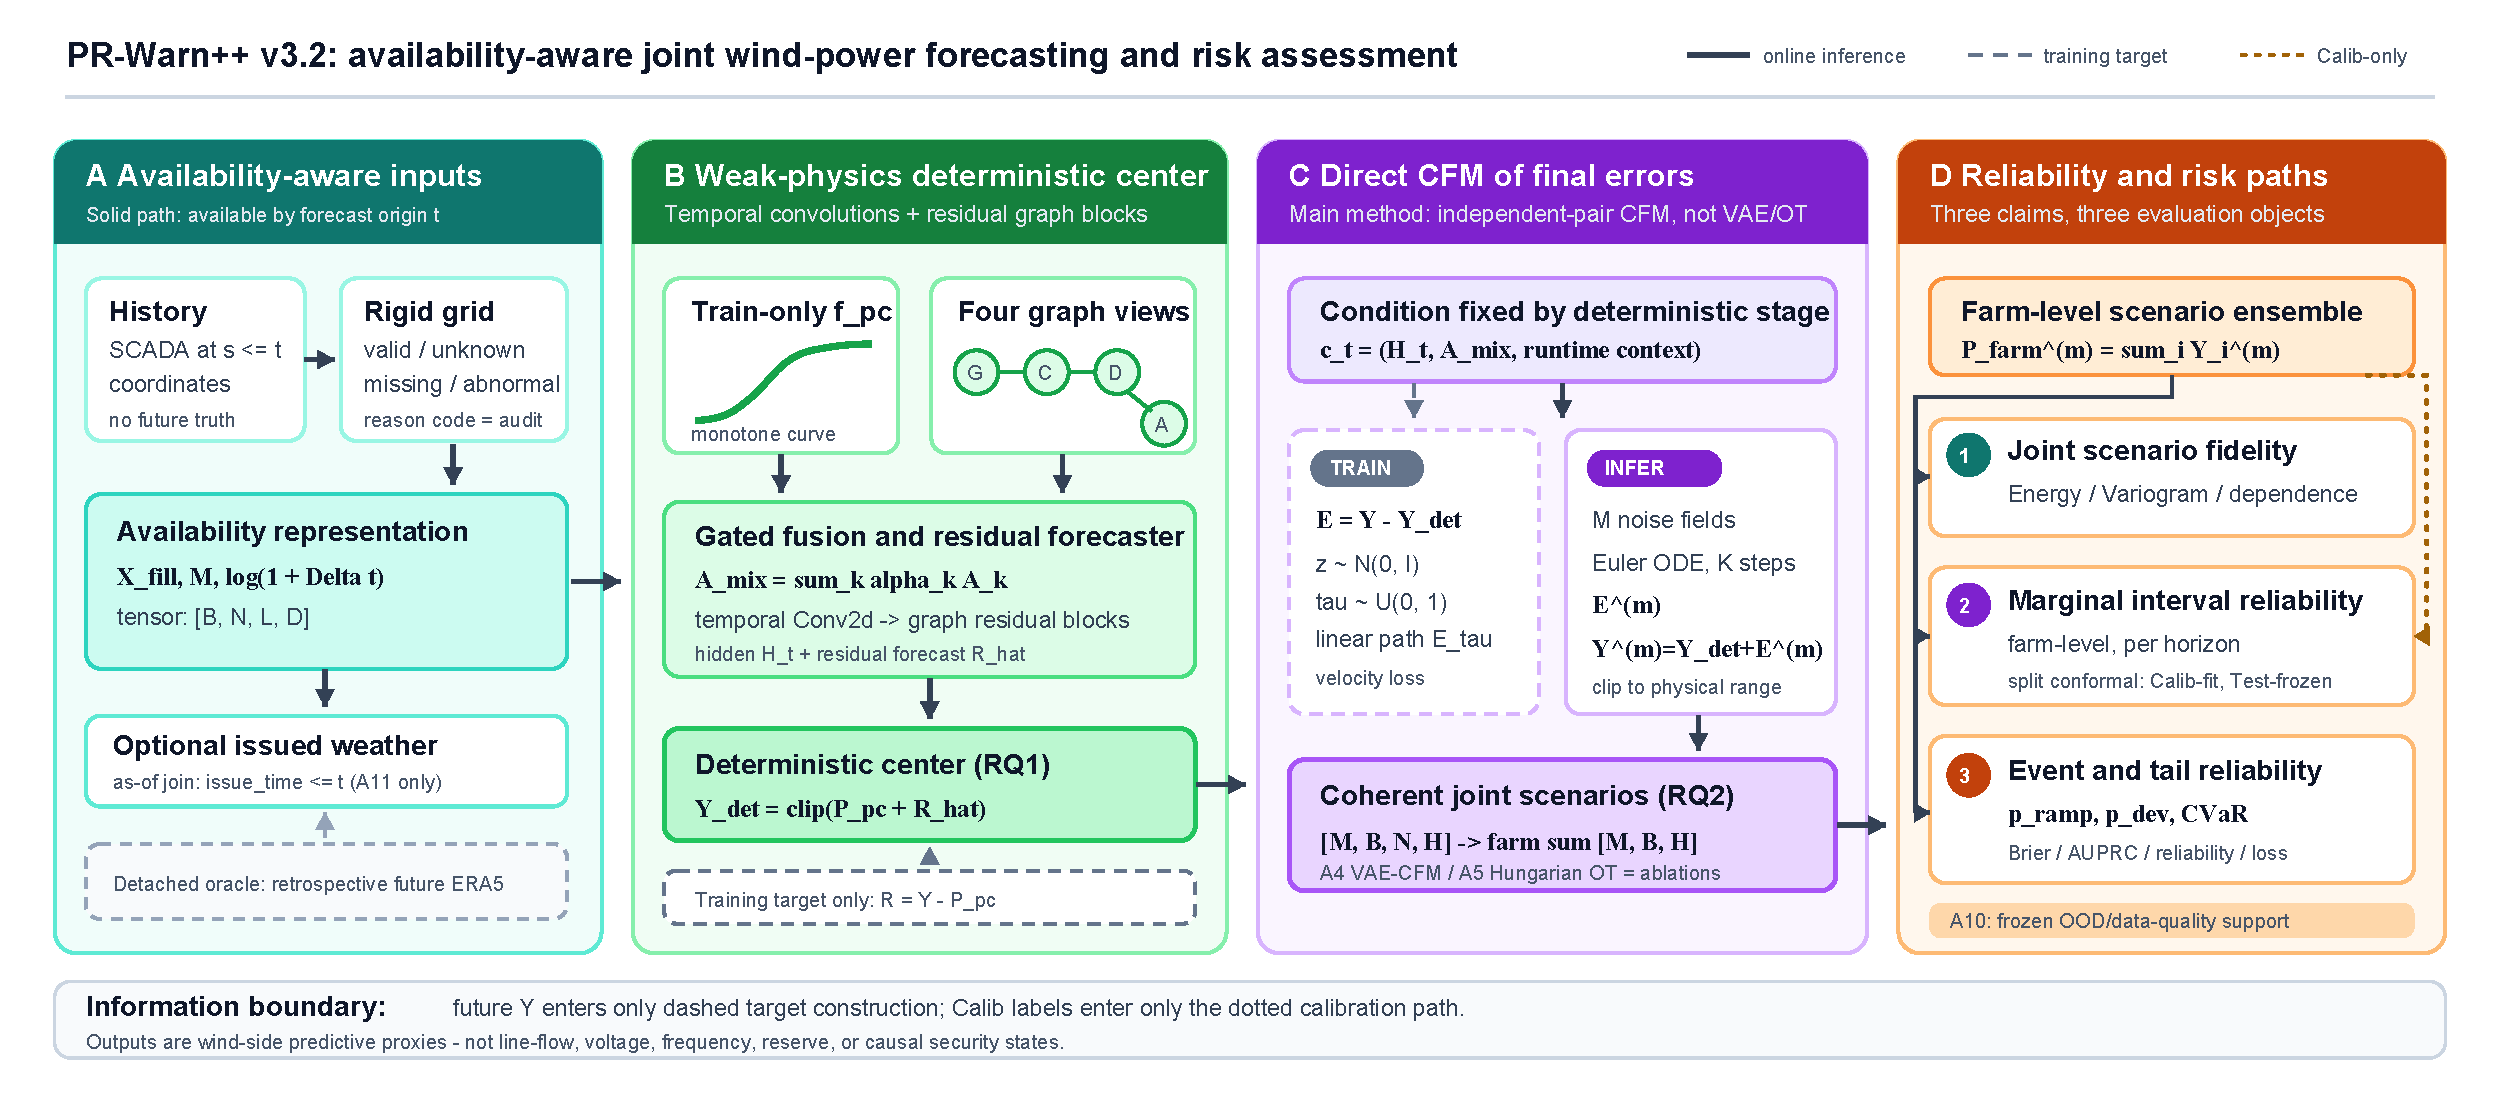
\includegraphics[width=0.985\textwidth]{prwarn_fig1_v3_2_vector.pdf}
\caption{PR-Warn++ v3.2 information architecture. Solid paths contain only information available at the forecast origin; dashed paths construct training targets; dotted paths are Calib-only; and the detached gray branch denotes retrospective oracle weather. The weak power-curve anchor and temporal multi-graph model form the deterministic center (RQ1). Direct CFM generates the joint final forecast-error field and reconstructs coherent power scenarios around the unchanged center (RQ2). Scenario fidelity, farm-level marginal conformal intervals, and event/tail-risk reliability are then evaluated as three distinct objects (RQ3).}
\label{fig:framework}
\end{figure*}

\section{Experimental Validation Protocol}

The primary benchmark is SDWPF-full \cite{zhou2024sdwpf}. The configured history and horizon are $L=24$ and $H=6$, corresponding to 240 min of history and 10--60 min forecasts. Chronological Train/Val/Calib/Test proportions are 60/15/10/15, subject to the final event-isolation and schema audit. SDWPF history-only is the main claim protocol, and future ERA5 is an oracle experiment. The WIND Toolkit contains retrospective meteorological and power reforecast products \cite{draxl2015windtoolkit,hodge2016windforecast}; it is only a candidate source for A11, which remains blocked until the selected archive exposes auditable issue and valid timestamps. Kelmarsh is reserved for external physical and data-quality validation \cite{plumley2025kelmarsh}.

Deterministic comparisons include persistence, the empirical anchor, controlled GRU/TCN models, Graph-WaveNet-style and AGCRN-style implementations, and the dynamic multi-graph residual model. The two style baselines share the same information and training contract and are not described as exact reproductions of external repositories. Probabilistic comparisons include Gaussian and Student-$t$ marginals, quantile/CQR, deep ensembles, Gaussian residuals, residual bootstrap, Gaussian copula, CVAE, DDIM, VAE-CFM, and Direct CFM. The A0--A11 and B0--B9 matrix fixes five seeds and separates target, graph, missingness, calibration, stress, risk-composition, and weather-protocol ablations.

Point accuracy is assessed with MAE and RMSE. Marginals use CRPS, pinball loss, PICP, width, and Winkler score. Joint scenarios use Energy and Variogram Scores \cite{gneiting2007proper,scheuerer2015variogram}. Ramp and deviation probabilities use Brier score, AUPRC, event F1, and reliability diagrams. Dependent-sample comparisons use paired day/event-block bootstrap intervals and HAC/Diebold--Mariano statistics. Inference reports scenario count, ODE steps, latency percentiles, throughput, parameter count, and peak VRAM. All of these are pending frozen-data/server measurement and are not treated as achieved results in this draft.

\section{Results and Discussion}

\TODO{Populate only from frozen five-seed server artifacts. Planned order: deterministic center and extreme regimes; marginal and joint probabilistic quality; ramp/deviation reliability; A0--A11 ablations; missingness stress; efficiency; and external validation. Every quantitative sentence must be traceable to an experiment ID and saved metric file.}

\section{Scope, Limitations, and Threats to Validity}

Future ERA5 is retrospective reanalysis and cannot support an operational NWP claim. The empirical curve is a weak reference, not a wake solver or aeroelastic model. Split-conformal coverage is marginal under the declared calibration protocol; ACI introduces online adaptation, while context/OOD fallback remains heuristic. Joint scenario quality must be established by proper multivariate scores and event reliability rather than interval coverage alone. Ramp, deviation, and CVaR outputs are wind-side proxies. Without network topology, load, dispatch, and dynamic models, they are not probabilities of line overload, voltage collapse, frequency instability, or reserve insufficiency. Finally, external datasets differ in turbine count, instrumentation, and weather availability, so conclusions must use shared semantics and normalized quantities instead of pooling incomparable absolute errors.

\section{Conclusion}

PR-Warn++ v3.2 separates an availability-aware weak-physics deterministic center from direct joint generation of the remaining final forecast-error field. It also separates three kinds of probabilistic evidence: joint scenario fidelity, marginal interval coverage, and event/tail reliability. The resulting formulation is deliberately auditable: history-only inputs define the primary claim, future ERA5 is isolated as an oracle, issue-time weather requires an as-of leakage gate, and risk outputs remain wind-side proxies. \TODO{After server validation, add the principal quantitative result, one efficiency result, and the strongest observed limitation.}

\section*{Acknowledgment}
\TODO{Funding, data-provider acknowledgment, and contributor statements.}

\bibliographystyle{IEEEtran}
\bibliography{prwarn_tste_v3_2_refs}

\end{document}
